\chapter{Introduction}

Les observations statistiques peuvent \'etre class\'ees en fonction de leur niveau, du plus particulier au plus g\'en\'eral:\\

\begin{defi}
Une \emph{unit\'e statistique} est le plus petit \'el\'ement sur lequel
porte l'analyse statistique.
\end{defi}
\begin{defi}
Une \emph{variable statistique} est une caract\'eristique d'une
unit\'e statistique.
\end{defi}
\begin{ex}
Unit\'e statistique: un(e) \'etudiant(e) de la HEG.\\
Variables: la couleur des yeux, la taille, le poids, le sexe, ....\\
\end{ex}

\begin{defi}
Une \emph{population} est un ensemble de toutes les unit\'es statistiques sur lequel porte une \'etude
statistique.
\end{defi}
\begin{defi}
Un \emph{\'echantillon} est un sous-ensemble de la population.
\end{defi}
Les donn\'ees r\'ecolt\'ees sont g\'en\'eralement issues d'un \'echantillon
d'\emph{individus} d'une population d'int\'er\'et.

\begin{ex}
Population: ensemble des \'etudiants de la HEG.\\
\'Echantillon: ensemble des \'etudiants de premi\`ere ann\'ee de la HEG.\\
Individu: un(e) \'etudiant(e) de premi\`ere ann\'ee de la HEG.
\end{ex}
On veut \'etudier une ou plusieurs caract\'eristiques que poss\`ede
chaque individu d'une population.

\begin{rem}
Lorsque les donn\'ees proviennent d'observations collect\'ees au m\^{e}me moment (ou presque), on parle de \emph{donn\'ees en coupe transversale}.
\end{rem}

{\bfseries \large Statistique descriptive}

En statistique descriptive, l'objectif est de d\'ecrire et comprendre les donn\'ees \`a disposition. Le niveau auquel elles appartiennent n'a pas alors beaucoup d'importance. Lorsque l'on travaille sur l'ensemble des donn\'ees d'une population, c'est parfois la seule phase statistique. L'analyse exploratoire sugg\`ere des hypoth\`eses de travail et des mod\`eles qui peuvent \^{e}tre formalis\'es et v\'erifi\'es en
statistique inf\'erentielle.

 \vspace*{2ex}

{\bfseries \large Statistique inf\'erentielle}

En statistique inf\'erentielle au contraire, on travaille toujours \`a partir d'un \'echantillon de donn\'ees issu d'une population que nous ne pouvons pas interroger ou examiner dans son ensemble, mais pour laquelle on aimerait disposer de r\'esultats fiables. Elle conduit \`a des conclusions statistiques \`a partir de donn\'ees en utilisant des notions de la th\'eorie des probabilit\'es. Cette partie s'occupe des m\'ethodes de test et d'estimation des param\`etres.

\begin{figure}[hbt]
\centerline{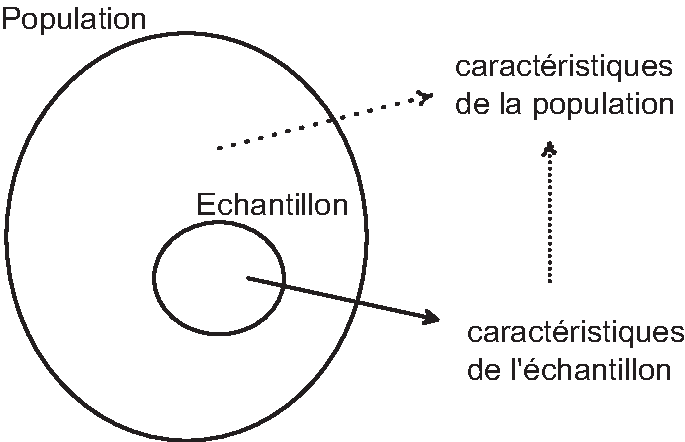
\includegraphics[scale=0.6]{inference}}
\caption{Principe de l'inf\'erence statistique}
\end{figure}

\begin{defi}
Un \emph{param\`etre} est une mesure calcul\'ee \`a partir d'une population enti\`ere.
\end{defi}

\begin{defi}
Une \emph{statistique} est une mesure calcul\'ee \`a partir d'un \'echantillon.
\end{defi}

Aussi longtemps que la population ne change pas, la valeur d'un param\`etre associ\'e \`a cette population ne varie pas. Par contre, la valeur d'une statistique d\'epend de l'\'echantillon s\'electionn\'e. Il existe donc g\'en\'eralement une diff\'erence entre la valeur d'un param\`etre, et son estimation par une statistique.

\begin{defi}
L'\emph{erreur d'\'echantillonnage} est la valeur de la diff\'erence entre une statistique et le param\`etre \'evalu\'e.
\end{defi}


% La statistique inf\'erentielle a les objectifs suivants:
% \begin{itemize}
% \item D\'eterminer des lois g\'en\'erales \`a partir d'un \'echantillon de donn\'ees.
% \item Estimer un param\`etre.
% \item Tester une hypoth\`ese.
% \item Evaluer la fiabilit\'e des r\'esultats.
% \end{itemize}
